\clearpage
\section{Omni-Channel}\label{hauptabschnitt_3}

\subsection{Welche Rolle spielt E-Commerce im Omni-Channel?}\label{unterabschnitt_3_1}
E-Commerce spielt eine wichtige Rolle im Omni-Channel-Ansatz, bei dem Unternehmen ihre Kunden und Kundinnen  über mehrere Kanäle hinweg ansprechen und interagieren. E-Commerce ist ein wichtiger Kanal, um Kunden und Kundinnen  online zu erreichen und ihnen Produkte und Dienstleistungen anzubieten.
\newline
Bei einem Omni-Channel-Ansatz besteht für Unternehmen ein Nebenziel darin, mittelfristig die Bekanntheit der eigenen Marke durch die Nebenwirkungen des Omni-Channel-Marketings auszubauen. Durch neue Point-of-Sale Möglichkeiten werden die Produkte und Dienstleistungen online angeboten. Dies ermöglicht es ihnen, die Kunden und Kundinnen auf verschiedenen Kanäle zu erreichen, zum Beispiel über ihre eigene Website, Social-Media-Plattformen oder Marktplätze wie Amazon.
\newline
Ein \ac{pos} ist ein Verkaufspunkt bzw. ein Ort, der es den Kunden und Kundinnen ermöglicht, ein Produkt zu kaufen. Im Allgemeinen bezieht sich der POS auf physische Verkaufsstellen, wie z.B. Ladengeschäfte, der POS kann sich aber auch auf Online-Verkaufsstellen, wie einen Marketplace oder einen Online-Shop beziehen\footnote{Vgl. \autocite [Online] {Kenning2018}}.
POS-Systeme bestehen aus Hardware und Software, die es dem Verkäufer ermöglichen, Artikel zu scannen, Zahlungen zu akzeptieren und Berichte zu erstellen und sie können zudem in andere Systeme wie Lagerverwaltung, Buchhaltung und CRM integriert sein.
\newline

E-Commerce ermöglicht es Unternehmen auch, ihre Kunden und Kundinnen über verschiedene Geräte hinweg anzusprechen, wie zum Beispiel Desktop-Computer, Laptops, Tablets und Smartphones. Auf diese Weise können Unternehmen ihre Kunden und Kundinnen  jederzeit und überall erreichen und ihnen eine nahtlose Einkaufserfahrung bieten.
\newline
Im Omni-Channel-Ansatz arbeiten E-Commerce und andere Kanäle wie der stationäre Handel, Kataloge und andere Marketing- und Verkaufskanäle zusammen, um eine umfassende Kundenerfahrung zu bieten. Kunden und Kundinnen  können zum Beispiel online recherchieren und dann im Ladengeschäft kaufen, oder umgekehrt. Unternehmen können auch eine integrierte Kundenbeziehung über mehrere Kanäle hinweg aufbauen und pflegen, indem sie Informationen und Interaktionen über alle Kanäle hinweg verfolgen und nutzen.
\newline

Eine repräsentative Studie des Handelsverband Deutschland von 2021 untermauert, dass der Online Einkauf in Deutschland nicht nur steigt, sondern dass der Einkauf über Smartphones immer häufiger genutzt wird und in den letzten Jahren kontinuierlich steigt. Diese Studie zeigt allerdings auch, dass Deutschland marketingtechnisch noch nicht auf dem Entwicklungsstand ist, wie es zum Beispiel Länder aus Asien sind (z.B. China oder Südkorea). In Deutschland zweifeln viele Unternehmen noch, innovative Projekte mit der Nutzung von Künstlicher Intelligenz in ihr Unternehmen zu integrieren. Rund 13\% der Unternehmen wenden demnach KI in Deutschland aktiv mindestens in einzelnen Bereichen an. Es sind zudem rund 15\% der restlichen Unternehmen bereit, KI in Zukunft einzuplanen, während über 72\% ohne KI planen\footnote{Vgl. \autocite [Online] {Handelsverband2021}}.
\begin{figure}[!ht]
    \centering
    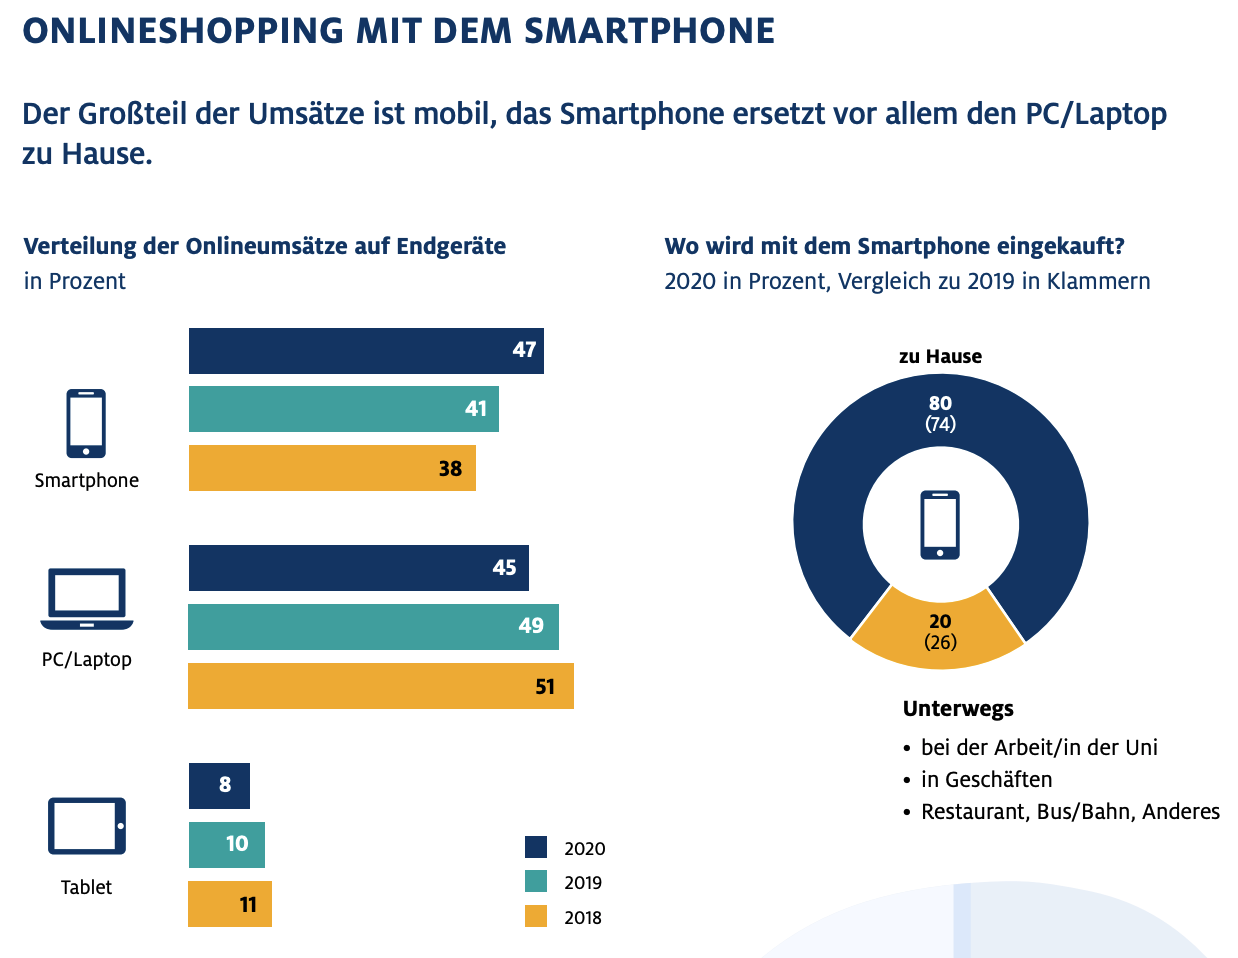
\includegraphics[width=0.95\textwidth,angle=0]{src/abbildungen/Shopping_smartphone.png}
    \caption[Quelle: HDE Deutschland Handelsverband - Marktentwicklung im Online-Handel, 2021]{Vgl.: Onlineshopping mit dem Smartphone, Quelle: \autocite {Handelsverband2021}}
   \label{Onlineshopping_smartphone}
   \end{figure}


\subsection{Wichtigkeit der Customer Journey}\label{unterabschnitt_3_2}
Als einer der ersten Menschen stellte Elmo Lewis bereits 1898 ein vier Stufen Modell auf, bei dem die Kunden und Kundinnen  vier Phasen bis zum Kauf des Produktes durchlaufen. Das sogenannte AIDA-Modell\footnote{Vgl. \autocite [Online] {Heubel2019}} beginnt damit, dass der Kunde oder die Kundin zum Beispiel durch Werbung auf ein Produkt aufmerksam gemacht werden soll (Awareness). Daraus resultiert ein Interesse des Betrachters, der sich mit dem Produkt oder der Werbung beschäftigt (Interest). Im dritten Schritt ist der Betrachter überzeugt von dem Produkt und hat den Wunsch, das Produkt zu kaufen (Desire).  In der vierten Phase wird das Produkt gekauft (Action).
\begin{figure}[!ht]
    \centering
    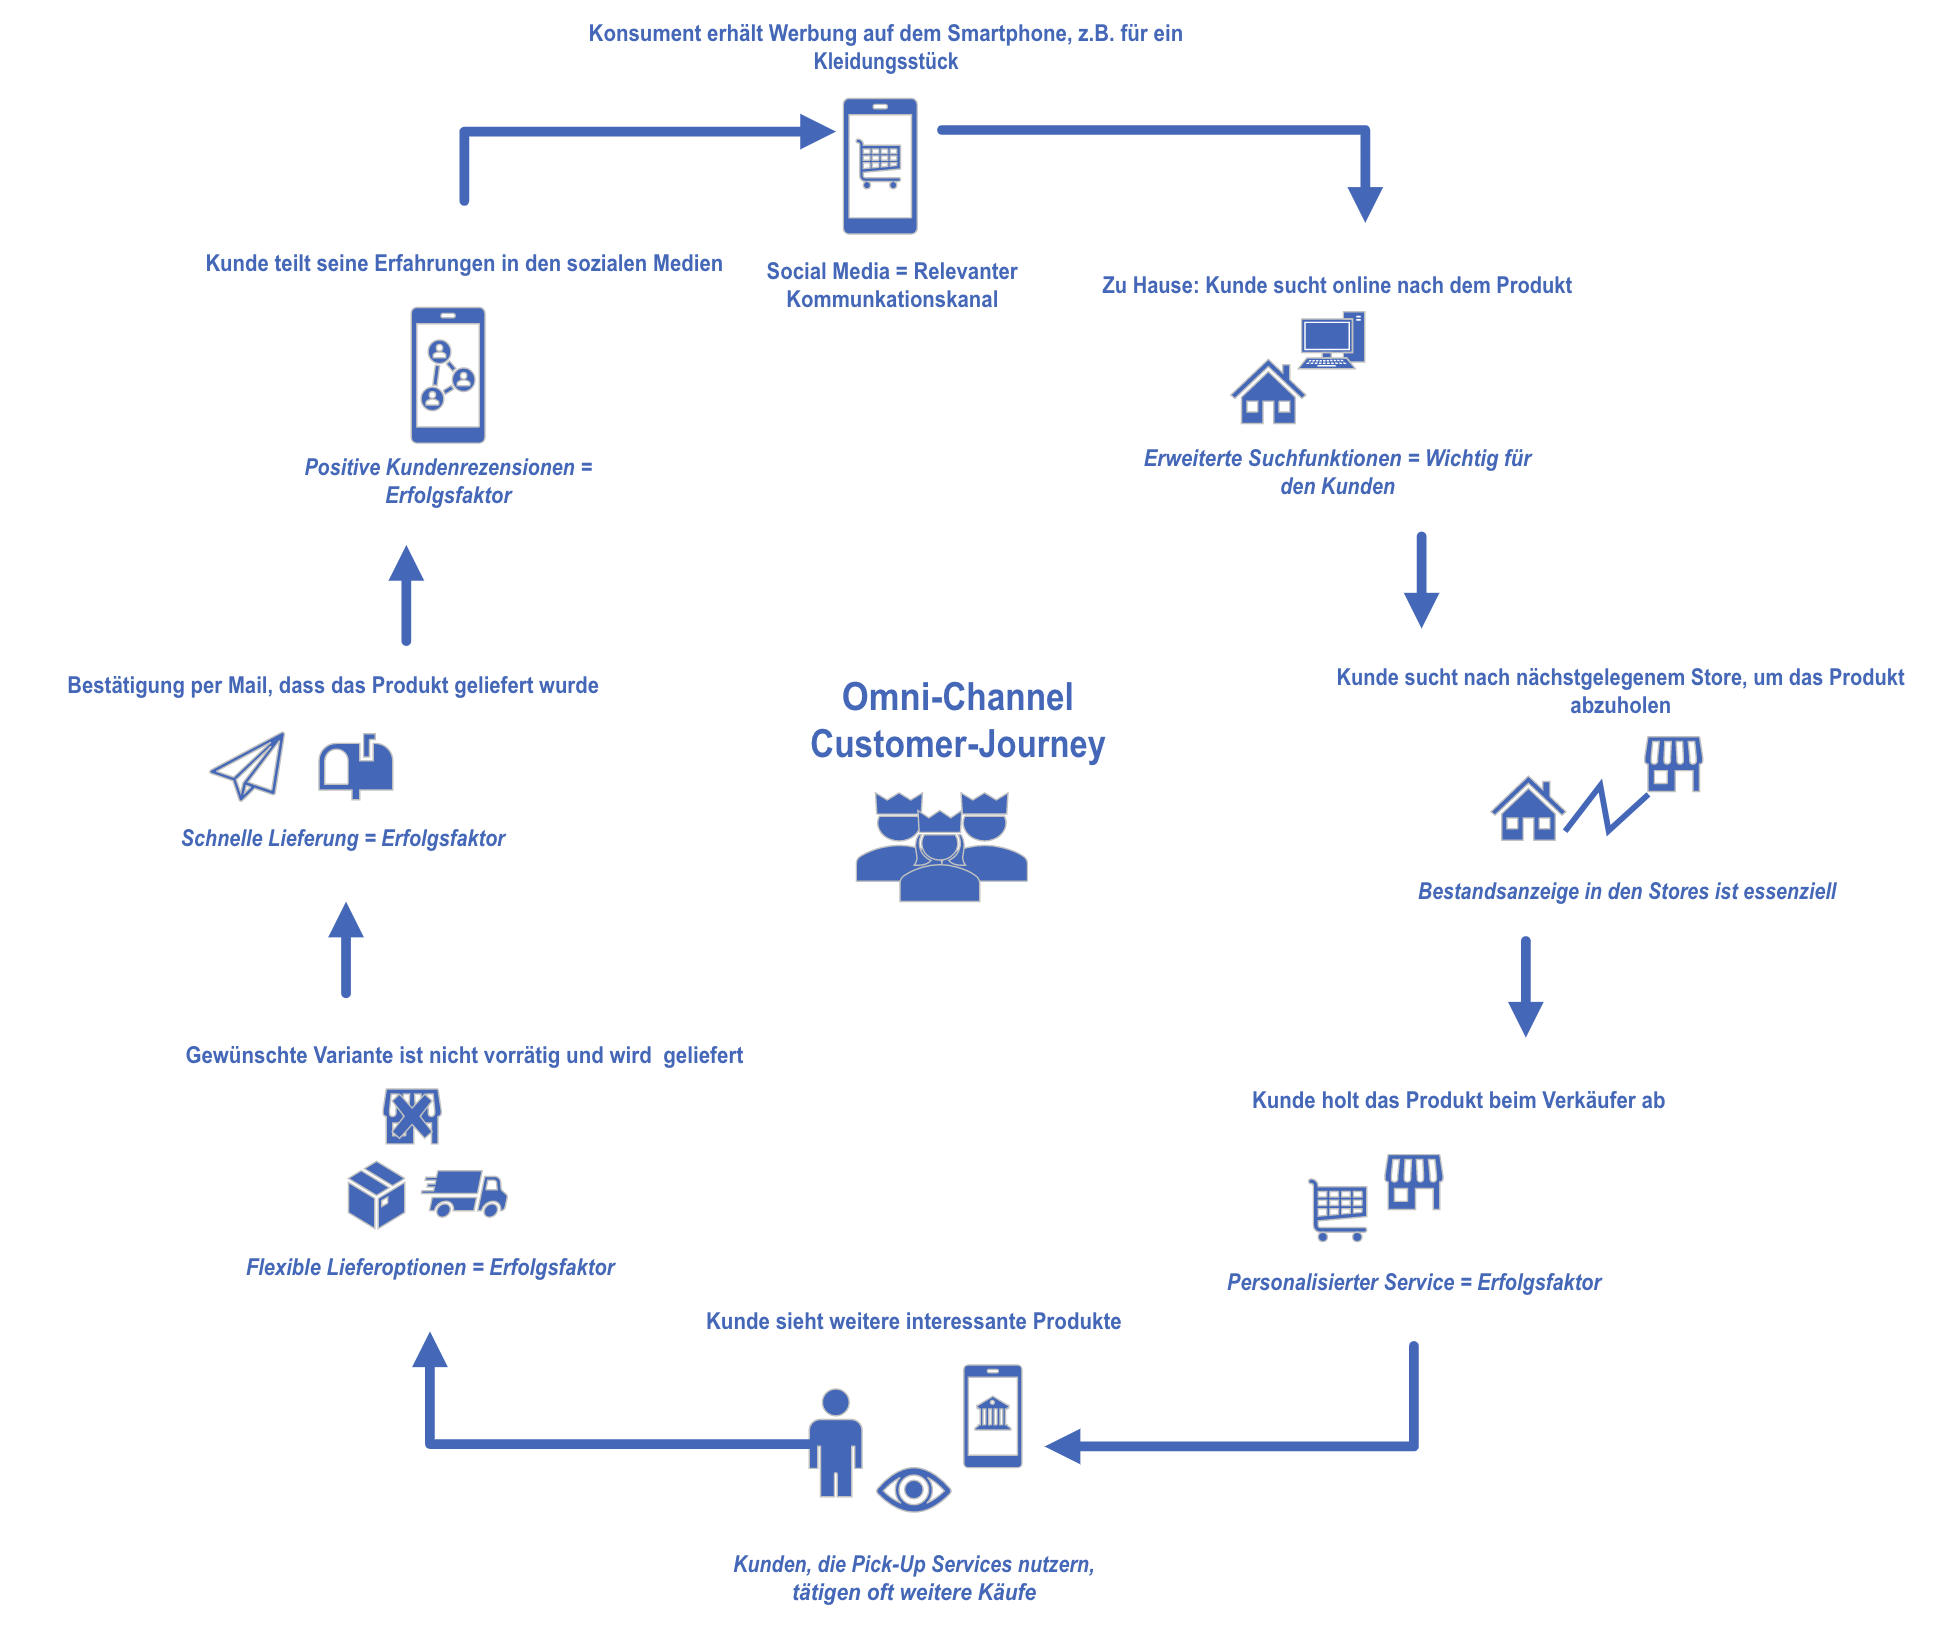
\includegraphics[width=0.95\textwidth,angle=0]{src/abbildungen/customer_journey.png}
    \caption[Quelle: Konzepte und Strategien für Omnichannel-Exzellenz S. 26, 2018]{Eine beispielhafte Customer Journey in Anlehnung an Böckenholt et all, Quelle: \autocite {Boeckenholt2018}}
   \label{customer_journey_2018}
   \end{figure}

\newpage
Die Customer Journey, also die Reise des Kunden oder Kundin, beschreibt den gesamten Prozess von der ersten Berührung, die der Kunde oder die Kundin mit dem Produkt widerfährt, bis hin zum Checkout, wo die Kaufabwicklung stattfindet.
\newline

Im Laufe der Customer Journey erreicht der Kunde oder die Kundin verschiedene Kontaktpunkte, sogenannte Digital Touchpoints. Durch die Auswertung der Digital Touchpoints können Informationen über den Kunden und Kundinnen gewonnen werden. Dieses Hintergrundwissen verbessert die Kundenberatung, die so proaktiv gestaltet werden kann. Durch die gewonnenen Informationen hat das Unternehmen die Möglichkeit, den Kunden oder die Kundin mit einer guten Beratung vom Produkt zu überzeugen\footnote{Vgl. \autocite [Online] {Duehning2021}}.
\newline

Im Normalfall entscheidet sich ein Kunde auch nicht direkt bei der ersten Berührung dafür, ein Produkt zu kaufen. Ein solcher Berührungspunkt in einem Einkaufsladen kann durch das Anschauen, das Sehen oder auch Riechen erfolgen. In der Regel gibt es zwischen Kunde und Produkt oder Marke mehrere Berührungspunkte, bis dieser überzeugt ist, das Produkt oder die Marke zu kaufen.
\newline

Eine Customer Journey von vor 10 Jahren ist jedoch nicht mehr mit einer Customer Journey von heute zu vergleichen, da sich die Einkaufsmöglichkeiten und die Verkaufskanäle im Laufe der Jahre durch die Digitalisierung verändert haben. Viele große Unternehmen haben bereits die Chance der technologischen Möglichkeiten ergriffen, den Kunden oder die Kundinnen einen nahtlosen Übergang der Verkaufskanäle anzubieten und die Customer Journey zu verbessern.
\newline

Dadurch, dass sich das Kaufverhalten enorm verändert hat und nicht mehr so linear verläuft, wie von dem AIDA-Modell dargestellt, entstanden einige neue Modelle, die eine Customer Journey beschreiben sollen. Als gemeinsamer Nenner wird bei diesen Modellen immer davon ausgegangen, dass die Kaufentscheidung ein Prozess ist, der nicht sofort getroffen wird. Dabei sollte berücksicht werden, dass durch die neuen Technologien (\ac{ua} KI) und Plattformen wie Social Media neue Phasen hinzu gestoßen sind.
\newline

Beim AIDA-Modell spielte der Prozess nach dem Kauf keine Rolle. Mundpropaganda und Meinungen über ein Produkt werden mittlerweile über Social Media Kanäle zum Beispiel von Blogger:innen und Influencer:innen heiß diskutiert und Bewertungen abgegeben.	 Nach dem Kauf kann man zwei Phasen ergänzend hinzufügen, wenn ein Unternehmen zum Beispiel bei einem Kunden oder einer Kundin nach dem Kauf nochmal explizit nach Feedback fragt und sichergeht, ob alles reibungslos bei der Lieferung abgelaufen ist und erfolgreich funktioniert. Wenn der Kunde mit dem Ablauf und dem Produkt zufrieden ist, führt dieses dazu, dass er in der Regel auch eher dazu tendiert, eine positive Bewertung für das Unternehmen abzugeben (Advocacy).
\newline

Ein Unternehmen, das die Customer Journey versteht, kann diese Kenntnisse nutzen, um gezielt im Marketing auf die Bedürfnisse und Präferenzen der Kunden einzugehen. Dies muss nicht zwangsläufig dazu führen, dass der Kunde das Produkt kauft, sondern kann dazu beitragen, verschiedene Ziele des Unternehmens zu erreichen, wie zum Beispiel das Abonnieren der Social-Media-Accounts, die Anmeldung für einen Newsletter, oder den Kauf eines anderen Produkts. Die Customer Journey bietet die Möglichkeit, die individuellen Ziele des Unternehmens zu verwirklichen\footnote{Vgl. \autocite [Online] {Gutmann2020}}.

\subsection{Customer Experience bei Omni-Channel-Strategien}\label{unterabschnitt_3_3}
Omni-Channel Kundenerfahrung (customer experience) bedeutet, dass ein Unternehmen Produkte und Kaufberatung über mehrere Kanäle an Interessenten und Kunden anbietet.
\newline
Jede Interaktion und jeder Berührungspunkt mit Kundenberater oder dem Produkt (soziale Medien, Chatbots, Kundenberatung) sind ein Teil dieser Customer Experience.
\newline

Der Omni-Channel-Ansatz ermöglicht es den Kunden und Kundinnen, die gesammelten Erfahrungen mit der Marke oder dem Produkt in einem Verkaufskanal zu beginnen und in einem anderen Kanal nahtlos fortzusetzen. Um dieses Ziel zu erreichen, müssen Unternehmen Ihre Marketing-, Vertriebs- und Kundensupport-Strategien aufeinander abstimmen.
\newline

Omni-Channel basierte Kundenerfahrungen (customer experience) sollten für Unternehmen kein Wunschtraum mehr sein. Für gut aufgestellte Unternehmen mit zukunftsorientiertem Denken ist es eine gute Chance, mit den neuen Technologien und Strategieansätzen die Verkaufskanäle noch stärker miteinander zu verknüpfen und neue Kunden-Features anzubieten. Mittel- und langfristig gesehen wird die Realität so aussehen, dass der Einsatz einer Omni-Channel-Strategie für Unternehmen mit mehreren Vertriebskanälen notwendig ist, um den modernen Verbraucher ansprechen zu wollen, da die Kundenbedürfnisse deutlich gestiegen sind und eine Customer Journey oft nicht mehr nur linear verläuft.
\newline

Das liegt daran, dass Verbraucher die Möglichkeit haben, eine ganze Reihe verschiedener Kanäle zu nutzen, um sich mit einer Marke oder einem Produkt auseinanderzusetzen und mehr zu erfahren. Beispiele sind die sozialen Medien, Videos, mobile Anwendungen oder die Google-Suche.
\newline

Omni-Channel-Kundenerlebnisse ermöglichen es Ihnen, den modernen Verbraucher an jedem Punkt seiner Reise zu erreichen, unabhängig davon, über welchen Kanal er zugreift. Dies wirkt sich positiv auf die Qualität der Kundeninteraktionen aus und führt zu einer stärkeren Kundenbindung. Die Einführung eines Omni-Channel-Ansatzes bringt sowohl für Kunden als auch für das Unternehmen eine Reihe von Vorteilen mit sich.
\newline

Sobald es zwischen den Konsumierenden und einem der Verkaufskanäle des Unternehmens die ersten Berührungspunkte gibt, erwartet der Konsumierende eine reibungslose Kundenerfahrung. Die Bereitstellung von unterschiedlichen Verkaufskanäle, die miteinander verknüpft sind und  mit denen der Konsumierende interagieren kann, hilft dabei, das Einkaufserlebnis so angenehm wie möglich zu gestalten, ohne dabei die Relevanz zu verlieren, dem Konsumierenden für das Produkt oder die Marke zu begeistern.
\newline

Mit Hilfe von Studien konnte gezeigt werden, dass die Kundenbindung und die Umsätze steigen, wenn mehrere Vertriebskanäle genutzt werden. Dabei haben Kunden und Kundinnen, die drei oder mehr Kanäle nutzen, um mit Marken zu interagieren, eine um 250 Prozent höhere Kaufhäufigkeit als Kunden, die nur einen Kanal nutzen. Die Harvard Business Review berichtet außerdem, dass Kunden, die mehr Kanäle nutzen, im Durchschnitt 4 Prozent mehr in Geschäften und 10 Prozent mehr online ausgeben.

\subsection{Äußere Einflussfaktoren}\label{unterabschnitt_3_4}
Äußere Einflussfaktoren müssen beim Omni-Channel-Retailing genauso berücksichtigt werden, wie die Anforderungen. Es handelt sich zwischen den Anforderungen und den äußeren Einflussfaktoren um ein Zusammenspiel, das sich in einem gegenseitigen Spannungsfeld befindet. Bei den äußeren Einflussfaktoren handelt es sich mit den Kundenanforderungen, Nachhaltigkeitsthemen und den technischen Entwicklungen um drei wichtige Faktoren, die für die Umsetzung einer Omni-Channel-Strategie berücksichtigt werden müssen\footnote{Vgl. \autocite [S. 26] {Vallee2018}}.
Durch die Nutzung neuer Technologien ist es möglich, dem Kunden oder der Kundin ein passendes Einkaufserlebnis zu verschaffen. Dafür wird im Verlauf dieses Abschnitts auf die technischen Prozesse eingegangen, die darstellen, wie ein solches Einkaufserlebnis personalisiert werden kann.

\subsubsection{Kundschaft im Zentrum}\label{unterabschnitt_3_4_1}
Beim Omni-Channel-Retailing spielen die Kundenanforderungen eine sehr wichtige Rolle. Diese Strategie zielt darauf ab, dem Kunden oder der Kundin ein nahtloses Einkaufserlebnis über alle Kanäle hinweg zu bieten. Dazu gehören sowohl Online- als auch Offline-Kanäle wie Filialen, Callcenter und Social Media.

\begin{figure}[!ht]
    \centering
    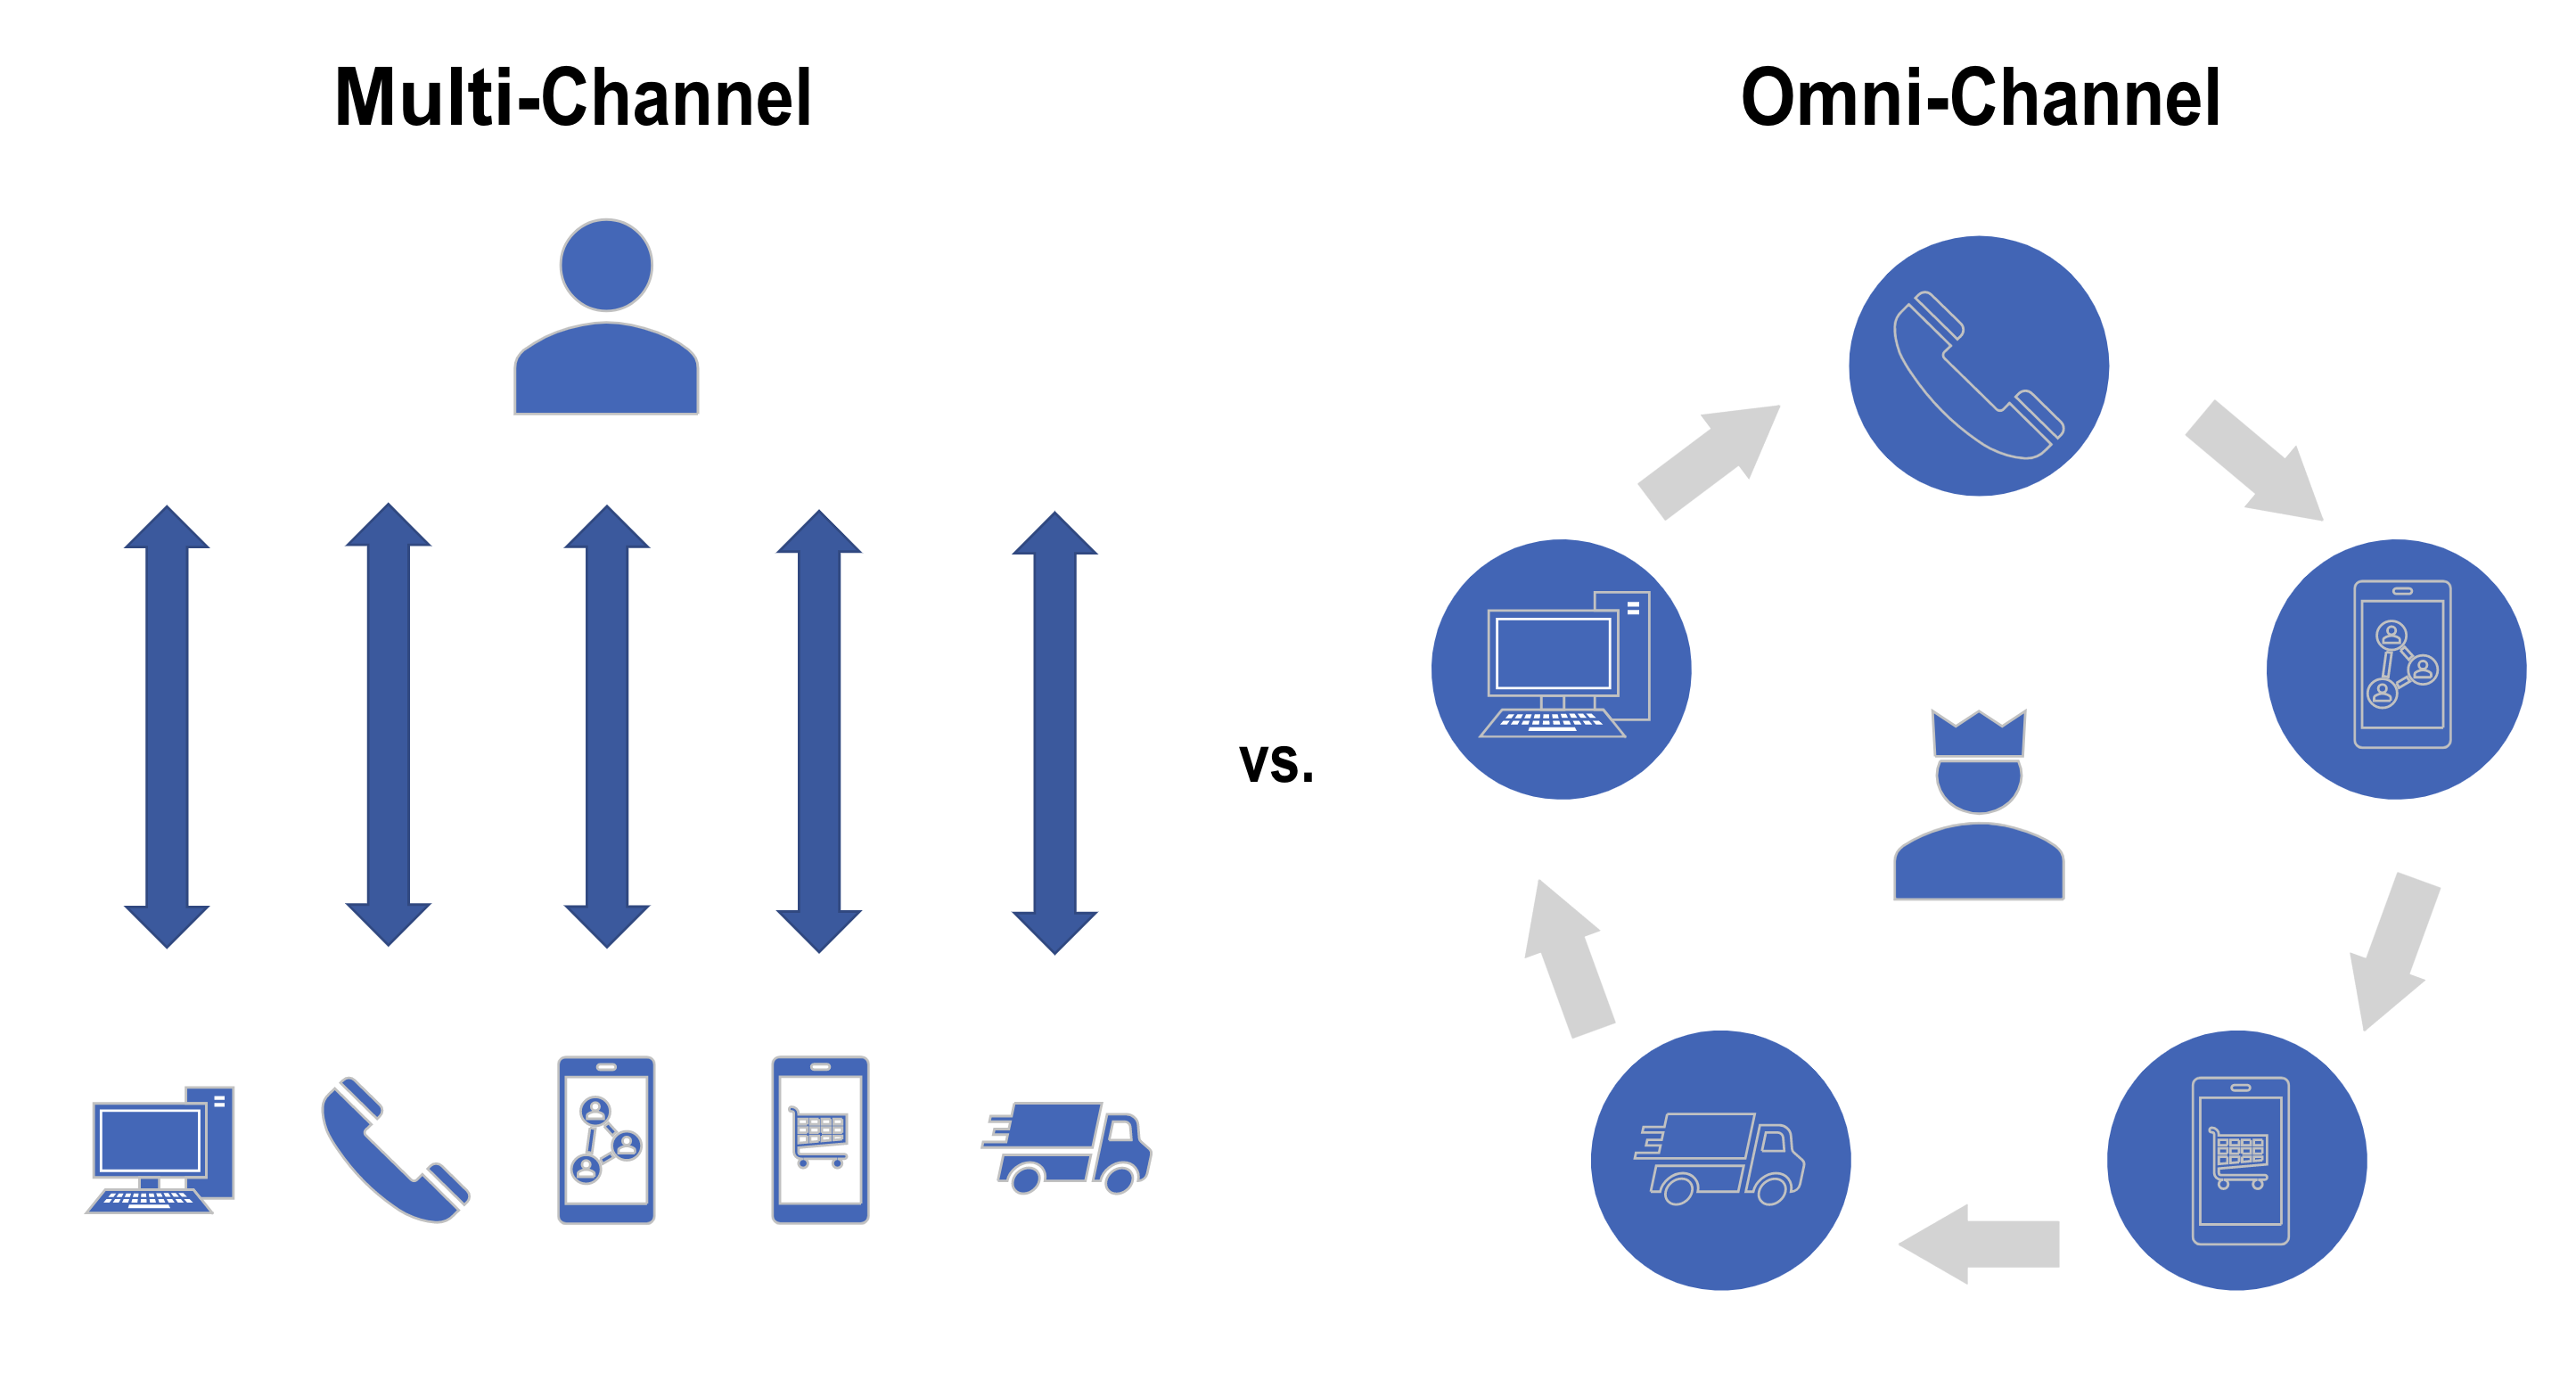
\includegraphics[width=1\textwidth,angle=0]{src/abbildungen/Multi-vs-Omni.png}
    \caption[Quelle: Omni-Channel Retailing S. 10, 2021]{Gegenüberstellung Multi-Channel-Marketing vs. Omni-Channel-Marketing in Anlehnung an Winters, Quelle: \autocite {Winters2021}}
   \label{fig: Quelle: omni_channel_retailing_2021}
   \end{figure}



Der Kunde oder die Kundin steht im Fokus der Omni-Channel-Strategie, da er oder sie auf allen verfügbaren Plattformen und in verschiedene Richtungen mit dem Unternehmen interagiert, um sich mit der Marke oder dem Produkt zu beschäftigen. Daher werden bei der Entwicklung einer Omni-Channel-Strategie die Bedürfnisse und Erwartungen der Kunden und Kundinnen sorgfältig analysiert und in den Prozess einbezogen. Ziel ist es, die bestmöglichen Angebote und Services bereitzustellen, die die Bedürfnisse der Kunden erfüllen und ihnen ein konsistentes und zufriedenstellendes Einkaufserlebnis bieten. Das bedeutet, dass ein Unternehmen die Präferenzen der Kunden in Bezug auf die Kanäle, die sie nutzen, um Produkte und Dienstleistungen zu erwerben und sich mit dem Unternehmen zu beschäftigen, berücksichtigen muss, um die bestmöglichen Ergebnisse zu erzielen. Es beinhaltet auch eine gute Kommunikation mit den Kunden und eine Möglichkeit für sie, ihre Erfahrungen und Bedürfnisse zu teilen, die wiederum für das Unternehmen wichtig sind, um sich weiter zu verbessern.
\newline

Eine erfolgreiche Omni-Channel-Strategie erfordert von Unternehmen die Schaffung von einem einheitlichen Kauferlebnis und einem konsistenten Erscheinungsbild. Damit eine solche Strategie erfolgreich umgesetzt werden kann, ist es wichtig, dass sowohl der Kunde als auch der Händler die volle Kontrolle über die Integration von Daten und Transaktionen haben, insbesondere in Bezug auf Preis, Lagerbestand, Lieferung und After-Sales-Service.
\newline
Bei dem Punkt Datenschutz treten jedoch vor allem im Internet große Probleme auf. Unternehmen müssen die Glaubwürdigkeit ihrer Kunden und Kundinnen gewinnen, damit diese sich auch bereit erklären, ihre Daten bereit zu stellen, so dass Unternehmen dann auch mit diesen Daten intelligent aufbereitet werden und für den Servicemitarbeiter zur Verfügung gestellt werden können.
Viele Konsumierende wären bereit, dem Unternehmen private Daten bereitzustellen. Das fehlende Vertrauen kommt jedoch daher, dass die Konsumierenden nicht wissen, was mit diesen Daten angestellt wird und die Konsumierenden am Ende des Tages nicht selbständig entscheiden können, was mit diesen Daten passiert. In diesem Fall muss der Prozess transparenter werden und die Konsumierenden müssen entscheiden können, was mit den Daten passieren darf.

Nach der Definition von Heinemann\footnote{Vgl. \autocite [S. 10] {Boeckenholt2018}} steht der Kunde oder die Kundin sogar vollständig im Fokus, wobei das Omni-Channel-Management nicht als Vertriebsstrategie, sondern als Verhaltensweise des Kunden betrachtet wird.
\newline

Kunden und Kundinnen nutzen heutzutage eine Vielzahl von Medien und Vertriebskanälen, weshalb sie ein konsistentes Kauferlebnis über alle Kanäle hinweg erwarten. Durch diese Entwicklung verschwinden die natürlichen Grenzen des Vertriebs und es ergeben sich für das Kundenbeziehungsmanagement neue Herausforderungen.
\newline

Eine wichtige Komponente einer erfolgreichen Omni-Channel-Strategie ist die Fähigkeit, die Präferenzen und Verhaltensweisen der Kunden und der Kundinnen zu verstehen und zu nutzen. Dies umfasst die Identifizierung von Mustern im Einkaufsverhalten, wie zum Beispiel welche Kanäle die Kunden am häufigsten nutzen, welche Art von Produkten oder Dienstleistungen sie am häufigsten kaufen und zu welchen Tageszeiten sie am aktivsten sind.
\newline

Basierend auf diesen Erkenntnissen kann ein Unternehmen die Angebote und Services an die Bedürfnisse der Kunden anpassen. Zum Beispiel, wenn die meisten Kunden und Kundinnen über Online-Kanäle einkaufen, kann ein Unternehmen seine Online-Präsenz verbessern, um diese Kunden besser zu bedienen. Wenn die meisten Kunden Produkte in einer Filiale kaufen, kann ein Unternehmen seine Filialen optimieren, um die Kundenerfahrung zu verbessern.
\newline

Eine Omni-Channel-Strategie erfordert auch die Fähigkeit, Daten über Kundeninteraktionen und Kundenaktivitäten über alle Kanäle hinweg zu sammeln und zu analysieren. Dadurch erhalten Unternehmen die Möglichkeit, ein vollständiges Kundenprofil zu erstellen und so ein personalisiertes Angebot und bessere Angebote und Dienstleistungen bereitzustellen. Omni-Channel-Retailing verbessert auch die Nutzung von Cross-Selling Angeboten, indem auf den Kunden zugeschnittene Angebote angeboten werden. Cross-Selling-Strategien sind in der Kosmetikbranche sehr verbreitet und es werden oft Produktlinien angeboten, die miteinander kombiniert werden können, um das bestmögliche Ergebnis zu erzielen. Beispielsweise kann ein Kosmetikunternehmen seinen Kunden, die eine Gesichtscreme kaufen, empfehlen, auch eine passende Augencreme oder eine Feuchtigkeitspflege zu erwerben. Durch ein personalisiertes Einkaufserlebnis kann zum Beispiel die eine bevorzugte Creme von der Lieblingsmarke des Kunden empfohlen werden.
\newline

Damit eine Omni-Channel-Strategie erfolgreich umgesetzt werden kann, muss das Unternehmen auch sicherstellen, dass alle Kanäle gut miteinander vernetzt sind und dass die Kunden nahtlos von einem Kanal zum anderen wechseln können. Dies bedeutet, dass Kundendaten und Kundeninformationen über alle Kanäle hinweg zentral gespeichert werden, um ein konsistentes und personalisiertes Einkaufserlebnis zu gewährleisten.

\subsubsection{Nachhaltigkeit mit Sicht auf die Kosmetikbranche}\label{unterabschnitt_3_4_2}
Heutzutage wird der Begriff Nachhaltigkeit in fast allen Branchen verwendet und hat in der Regel eine positive Konnotation. Dieser Begriff wird häufig mit ökologischem Wirtschaften, nachhaltiger Nutzung von Rohstoffen und umweltfreundlicher Produktion in Zusammenhang gebracht.
\newline

Aufgrund der Vielzahl verschiedener Anwendungsbereiche gibt es keine einheitliche Definition von Nachhaltigkeit. Es handelt sich um eine Reihe von Denkansätzen und Strategien, wie zum Beispiel "die Sicherung der menschlichen Existenz, die Erhaltung des gesellschaftlichen Produktivpotenzials und die Gewährleistung von Handlungs- und Entwicklungsmöglichkeiten für die heutigen und zukünftigen Generationen"\footnote{\autocite [S. 18] {Pufe2017}}.
\newline

Nachhaltigkeit ist in der Kosmetikbranche zu einem wichtigen Thema geworden. Immer mehr Menschen wollen sicher sein, dass die Produkte, die sie verwenden, nicht nur gut für ihre Haut, sondern auch für die Umwelt sind. Unabhängige Gütesiegel wie das BDIH-Prüfzeichen (Bundesverband deutscher Industrie- und Handelsunternehmen) gestalten den Kaufprozess transparenter und ermöglichen es dem Kunden nachzuvollziehen, ob ein Produkt nachhaltig produziert wurde\footnote{\autocite [Online] {Flatley2021}}.
\newline

Eine nachhaltige Kosmetikbranche ist eine, die umweltfreundliche und ethisch vertretbare Praktiken anwendet und sich verantwortungsbewusst gegenüber Menschen und Natur verhält. Dazu gehört zum Beispiel, dass Rohstoffe möglichst lokal und biologisch angebaut werden und der Einsatz von Mikroplastik vermieden wird.
\newline

Ein weiterer wichtiger Aspekt ist die Verpackung von Kosmetikprodukten. Es gibt mittlerweile viele Unternehmen, die auf umweltfreundliche Alternativen wie Glas oder Papier setzen, anstatt Plastikverpackungen zu verwenden. Es ist wichtig, dass möglichst jedes einzelne Unternehmen in der Kosmetikbranche ihren ökologischen Fußabdruck minimiert und gleichzeitig hochwertige, sichere und wirksame Produkte anbietet, um auch langfristig erfolgreich zu sein und einen wichtigen Beitrag zu einer nachhaltigen Zukunft leisten.
\newline

Tierversuche spielen für die Nachhaltigkeit in der Entwicklung von Kosmetikartikeln ebenfalls eine wichtige Rolle. Tierschutzorganisationen wie PETA haben viele Jahre dafür gekämpft, dass Tierversuche in der Kosmetikbranche verboten werden\footnote{\autocite [Online] {PETA2021}}.
Für einen Großteil der Kosmetikartikel ist das mittlerweile der Fall. Tierversuchsfreie Produkte werden von Unternehmen auch als Verkaufsargument genutzt, denn heutzutage fordert ein Großteil der Konsumierenden in der Kosmetikbranche Nachhaltigkeit bei Kosmetikprodukten. Eine repräsentative Studie der globalen Strategieberatung Simon-Kutcher \& Partners vom Januar 2022 hat gezeigt, dass 58\% der befragten Konsumierenden in der \acs{dach}-Region darauf Wert legen, dass Kosmetikartikel nachhaltig hergestellt wurden\footnote{\autocite [Online] {Simon2021}}. Mit nachhaltigen Produkten können sich Unternehmen nach außen besser und erfolgreicher vermarkten.
\newline

Das Kosmetik-Unternehmen BABOR setzt sich bereits seit Jahrzehnten das Ziel, nachhaltig zu Wirtschaften und bestehende Prozesse nachhaltig zu überprüfen, um noch bessere Alternativen zu entwickeln. Das Unternehmen legt dabei ein besonderes Augenmerk auf die Abwasserreinigung und Mülltrennung. BABOR stellt in regelmäßigen Abständen einen Plan, der über 5 Jahre zieht, auf und legt dabei fest definierte Ziele fest, die nachvollziehbar und ergebnisorientiert sind. Vor allem die Bereiche Verpackung und Zutaten sind ein sehr großes Thema, was die Produktion angeht. BABOR setzt und auch das Ziel, bis 2025 im Bereich des Green Packaging, der Verwendung von reinen Inhaltsstoffen und die Entstehung von CO²-Emissionen aktiv zu vermeiden, indem auf Öko-Erdgas, Photovoltaik Anlagen und Ökostrom gesetzt und klimaneutral gearbeitet wird, also weitestgehend auf Plastik verzichtet wird und Alternativen genutzt werden.  Auch der Bereich der Elektromobilität wird von BABOR gefördert\footnote{\autocite [Online] {BABOR2022}}.

\subsubsection{Technische Entwicklung}\label{unterabschnitt_3_4_3}

Welche technischen Prozesse werden bei einer Omni-Channel-Strategie angewendet? Was gibt es für Möglichkeiten und wie verläuft eine Kanalintegration?
\newline

Die Kundenanforderungen haben ein Level erreicht, in dem die Möglichkeit auf barrierefreies Einkaufen mit nahtlosem Wechsel zwischen den Verkaufskanälen und einer passenden Beratung zu den Produkten von vielen modernen Kunden gefordert wird. Unternehmen müssen versuchen, diesen Forderungen gerecht zu werden, um eine Marke oder ein Produkt langfristig erfolgreich vermarkten zu können.
\newline

Eine Grundvoraussetzung liefert ein zentrales Order Management System (OMS), das sämtliche Daten, die das Unternehmen betreffen, kanalübergreifend miteinander synchronisieren kann.

\begin{figure}[!ht]
    \centering
    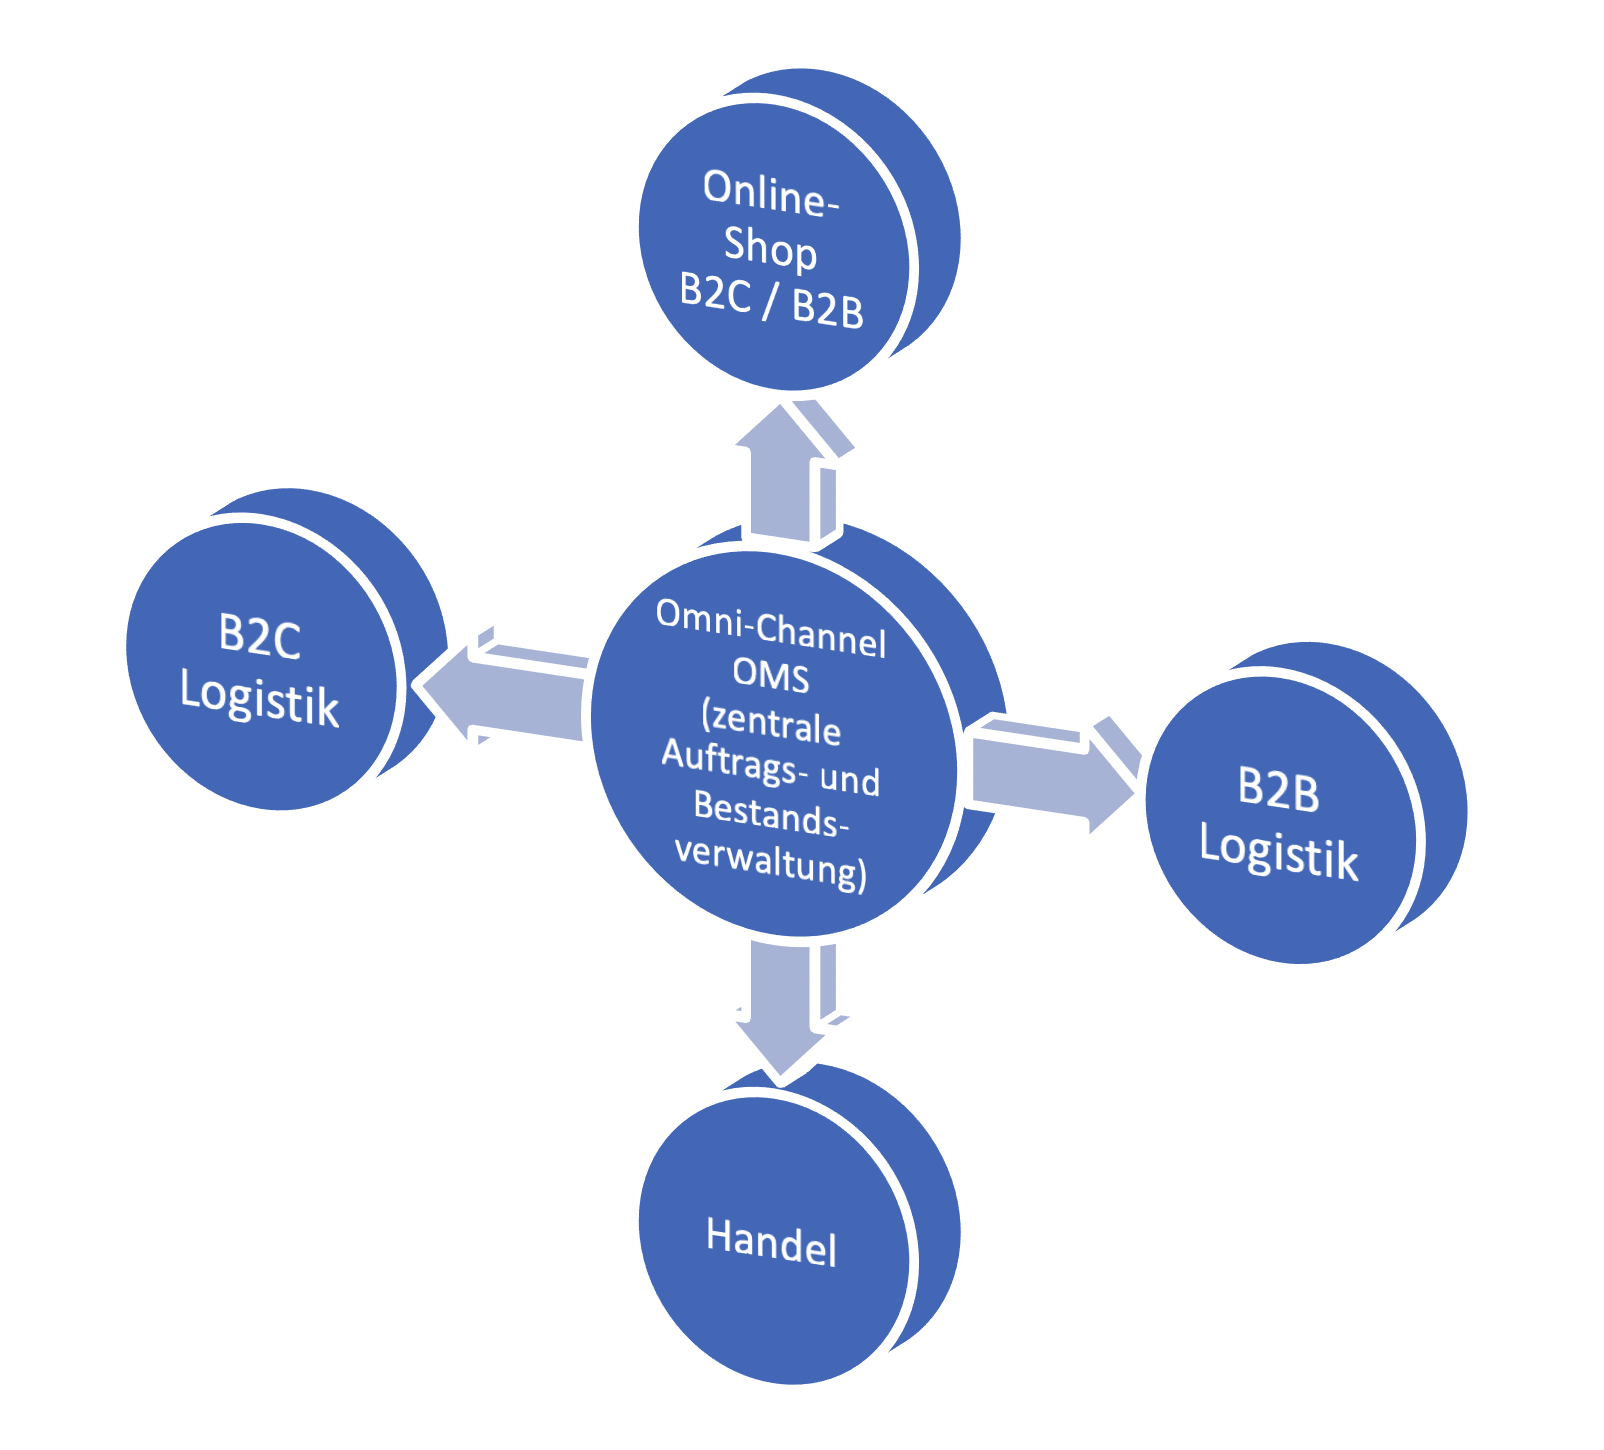
\includegraphics[width=1\textwidth,angle=0]{src/abbildungen/OMS-System.png}
    \caption[Quelle: Omni-Channel im Handel, 2018]{Zentrale Integrierung eines Order-Management-Systems in das Omni-Channel-Marketing in Anlehnung an Vallée et al, Quelle: \autocite {Vallee2018}}
   \label{fig: oms_system}
   \end{figure}

Dieses System bietet eine Schnittstelle für Verkaufskanäle, so dass diese ihre Daten miteinander synchronisieren können und Echtzeit Abfragen über aktuelle Bestände stattfinden können. Um die Möglichkeiten zu erweitern, kann das Kassensystem des Filialgeschäfts ebenfalls an das IT-System verknüpft werden, so dass kanalübergreifende Umsatzabfragen und Auswertungsmöglichkeiten bestehen.
\newline

Dort werden dann auch aufgezeichnete Daten mit Hilfe von Big Data Technologien gespeichert, die Informationen zu Kundengruppen oder auch einzelnen Kunden geben sollen. Big Data sind eine Vielzahl gesammelter Rohdaten, die Informationen über das Kauf- und Konsumverhalten von Konsumierenden liefern können. Diese Daten müssen verarbeitet werden, so dass Nutzdaten herausgefiltert und analysiert werden\footnote{\autocite [S. 6] {Fasel2016}}.
\newline

Mit Hilfe passender Software können Mitarbeiter die Informationen nutzen, um auf die Kundenbedürfnisse reagieren zu können und entsprechende Handlungsempfehlungen auszusprechen\footnote{\autocite [S. 28] {Vallee2018}}. Auch für den Bereich Marketing nimmt Big Data eine hilfreiche Rolle ein, indem zum Beispiel Auswertungen über Verkäufe über die Social-Media-Kanäle oder den Online-Shop getätigt werden können und Trends aufgezeigt werden.
\newline

Die Umsetzung für eine reibungslose und angenehme Auftragsabwicklung wird bei einem Omni-Channel-Retailing als Omni-Channel Fulfillment bezeichnet. Es kann vorkommen, dass einige Unternehmen für diesen Prozess oder bestimmte Teilaufgaben dieses Prozesses einen Logistikdienstleister beauftragen. Dazu gehören unter anderem die Produkte bzw. Waren, die kommissioniert, verpackt und an den Endkunden verschickt werden, aber auch die Abwicklung von Retouren.
\newline

Ein Unternehmen muss dabei abwägen, wie es strukturell aufgestellt ist, welche Kapazitäten zur Verfügung stehen oder wie groß die Lagerflächen sind. Daher kann es in bestimmten Fällen finanziell ein Vorteil sein, diese Aufgaben an einen Dienstleister abzugeben und sich so auf andere Kernpunkte wie den Service zu fokussieren. Weitere Teilprozesse, die das Omni-Channel-Fulfillment komplettieren, sind ein gut organisierter Check-Out-Prozess mit angenehmen Point-of-Sale Möglichkeiten und verschiedenen Lieferangeboten.
\newline

Gerade im Onlinebereich können dem Kunden über den POS eine Vielzahl von Optionen angeboten werden, um einen Kauf abzuschließen. Beispielsweise kann über ein geeignetes Shopsystem bei einer Onlinebestellung die Kaufabwicklung eines Stammkunden angenehmer gestaltet werden, indem die vorausgewählte Zahlungsart erkannt und automatisch hinterlegt ist oder passende Cross-Selling Angebote vorgeschlagen werden. Zudem erleichtert es dem Unternehmen, den Verkauf über mehrere Kanäle hinweg zu verfolgen und zu verwalten.
\newline

In der Kosmetikbranche nutzen bereits große Unternehmen die digitalen Möglichkeiten, um Kunden für sich zu gewinnen, indem sie ihre Produkte kanalübergreifend über ihren Online-Shop, einen Marketplace und in der Filiale verkaufen und gleichzeitig einen attraktiven Service anbieten. Dieser kann zum Beispiel Click \& Collect, Reserve \& Collect oder Return-to-Store Service sein. Bei dem Click \& Collect wird ein Einkauf online getätigt, beispielsweise über den Online-Shop und die Ware kann vor Ort in einer Filiale abgeholt werden\footnote{\autocite [S. 56] {Vallee2018}}.
Reserve \& Collect bietet dem Kunden die Möglichkeit, die Ware im Online-Shop zu reservieren und vor Ort am Point-of-Sale zu bezahlen und direkt mitzunehmen. Das Return-to-Store Angebot bietet dem Käufer bei einer Retoure die Möglichkeit, die online gekaufte Ware vor Ort in der Filiale umzutauschen.

\subsection{Potenziale und Herausforderungen des Omni-Channel}\label{unterabschnitt_3_5}
Die Digitalisierung hat nicht nur Auswirkungen auf den Handel. Durch die neuen Technologien entstehen tiefgreifende Veränderungen in der Denkweise der Gesellschaft. Deshalb müssen sich die Prozesse in Handelsunternehmen grundlegend anpassen und optimieren, um auf aktuelle und zukünftige Herausforderungen im Onlinehandel vorbereitet zu sein. Daraus können dann wiederum neue Türen geöffnet und neue Absatzgebiete erschlossen werden.
\newline

Die Vertriebsmöglichkeiten über den E-Commerce haben sich gefestigt und darüber hinaus sind sie mittlerweile in jedem großen Unternehmen ein fester Bestandteil der Unternehmensstruktur. Auch die Konsumierenden haben sich an die neuen Möglichkeiten gewöhnt und erwarten unter anderem permanente Verfügbarkeit der Online-Kanäle\footnote{\autocite [S. 426] {Heinemann2016}}.
\newline
Eine große Herausforderung stellt die Einrichtung der IT-Infrastruktur dar, die die verschiedenen Vertriebskanäle miteinander verschmelzen lassen und so einen nahtlosen Übergang der verschiedenen Kanäle garantieren soll.
Für die Anwendung einer Omni-Channel-Strategie ist eine zielgenaue Planung erforderlich. Daten über das Kaufverhalten der Kunden müssen gesammelt werden, um das Ziel, den Kunden in den Mittelpunkt zu stellen, erreichen zu können. Es gilt dabei herauszufinden, wie die Kunden ein Produkt kaufen wollen und welche Vertriebswege dabei für sie relevant sein können.
\newline

Bei der Planung werden Unternehmensstrukturen durchleuchtet und mögliche Anforderungsfälle erstellt. Zu einem solchen Prozess gehören nicht nur der Weg bis zum Warenkorb, sondern darüber hinaus auch Möglichkeiten, den Kunden zu unterstützen. Beispiele sind der Service, Vertrieb oder ein Produkt-Team.
\newline
Auch wenn das Live-System, auch Produktivsystem oder Produktivumgebung genannt, für die Verarbeitung der Software und den Quellcode des Online-Shops zuständig ist und damit das Herzstück für den Online-Shop darstellt, gibt es bei einer Omni-Channel-Strategie eine einzige Zentrale, die alle Verkaufskanäle miteinander verknüpfen soll. In den meisten Fällen nutzen Unternehmen dabei nicht den Online-Shop direkt, sondern eine \ac{erp}- und Warenwirtschafts-Lösung als Hauptquelle. Diese vereinfacht den Händlern unter anderem das Importieren und Migrieren von Produkten oder anderen Daten in den Online-Shop.
\newline
Die ERP- und Warenwirtschafts Lösung sorgt dafür, die betriebliche Effizienz zu verbessern, indem sie die Datenverwaltung zentralisiert, die Logistikprozesse optimiert und damit die Rentabilität erhöht und die Entscheidungsfindung erleichtert, indem sie mehr Transparenz bietet. In diesem Zusammenhang ist es genauso wichtig, die Schnittstellen so zu konfigurieren, dass die Datenintegrität reibungslos verlaufen kann und vollständig und korrekt konfiguriert wurde, um weitreichende Konsequenzen zu vermeiden, indem Informationen falsch weitergeleitet werden. Beispiele können Gutscheine oder Rabattaktionen sein, die kanalübergreifend funktionieren müssen, ohne Fehler zu produzieren. Das Controlling sollte dabei zentralisiert erfolgen.
\newline
Für neue Updates, Releases, aber auch mögliche Serverausfälle oder andere Infrastruktur-Ausfälle muss die Abteilung, die für die IT-Infrastruktur zuständig ist, möglichst präventiv oder schnell reagieren können, um Ausfallzeiten zu vermeiden und im besten Fall zu verhindern. Dieser Service für Wartung und das Entwickeln neuer Features oder Sicherheitsupdates für den E-Commerce Bereich wird in der Kalkulation für die Entwicklung eines Online-Shops bereits mit eingeplant. Bei der Verknüpfung der verschiedenen Verkaufskanäle wird der Umfang der Arbeit jedoch nicht geringer, es müssen noch mehr Prozesse berücksichtigt und eingebaut werden.
\newline

Dadurch lässt sich bereits erahnen, dass ein Unternehmen ein bestimmtes Budget investieren muss, um eine Omni-Channel-Strategie zu implementieren. Eine entscheidende Rolle spielt dabei auch die Größe des Unternehmens und wie viele Bestellungen in etwa pro Tag verschickt werden. Auch der Prozess beim Paketversand kann entsprechend optimiert werden.
\newline

Grundvoraussetzung für die Umsetzung einer Omni-Channel-Strategie ist für ein Unternehmen geeignetes Personal und Know How, um das Gerüst zu schaffen und eine Verkaufskanal übergreifende Infrastruktur aufzubauen. Zudem müssen alle Mitarbeiter geschult werden, um zu lernen, wie die Software funktioniert und genutzt werden kann.
\newline

Aus Käufersicht wird es ein wichtiger Punkt sein, den Point-of-Sale zum \ac{pop}, also dem Ort des Kaufs, umzugestalten. Entgegen dem POS agiert der POP nach dem Pull Prinzip. Dieses Prinzip wird als Pull-Prinzip bezeichnet, weil der Verkäufer keine Überzeugungsarbeit leisten muss, damit der Käufer ein Produkt aus Eigeninitiative aus dem Lager zieht. Der POP lässt sich auch im Online-Shop integrieren, indem zum Beispiel ein besonderes Produkt direkt auf der Hauptseite des Unternehmens besonders hervorstechen kann und so die Aufmerksamkeit des Konsumierenden auf sich ziehen kann.
\newline

Eine repräsentative Online Befragung von 2017 zeigte bereits einen Trend auf, dass obwohl die meisten deutschen Internetnutzer:innen den Einkauf im Geschäft bevorzugen, 70\% von ihnen mindestens einmal im Monat online einkaufen. Die Grenzen zwischen Online- und Offline-Käufen verschwimmen, da viele Käufer:innen ihr Smartphone nutzen, um sich über Produkte zu informieren und Coupons in Apps nutzen, um im Geschäft einzukaufen. Um die Konsumierenden effektiv anzusprechen, müssen Marken digitalen Content mit den stationären Einkaufserlebnissen verknüpfen\footnote{\autocite [Online] {Ipsos2017}}.
\newline

Gleichzeitig zeigt sich aber auch, dass Smartphones für Unternehmen eine wichtige Möglichkeit bieten, den Konsumierenden in einem entscheidenden Moment zum Kauf zu bewegen. Viele deutsche Online-Käufer:innen suchen bereits nach Produkten auf ihren Smartphones, nachdem sie Werbung gesehen haben, und mehr als die Hälfte der deutschen Onlinekäufer:innen kauften bereits 2017 über Apps auf ihrem Smartphone oder Tablet ein. Eine mobile Präsenz und Kommunikation ist daher ein wichtiger Faktor für Marken, um die Kundenbindung zu stärken und den Umsatz zu erhöhen. Personalisierte Push-Benachrichtigungen auf Basis der Daten der Benutzer:innen können die Aufmerksamkeit von Smartphone-Besitzern auf die Marke lenken, jedoch wird dieses Potenzial noch nicht ausreichend genutzt.
\subsection{Intralogistik}\label{unterabschnitt_3_6}
Die Intralogistik bezieht sich auf die innerbetrieblichen Prozesse der Materialwirtschaft und der Logistik. Im Zusammenhang mit dem Omni-Channel-Marketing in der Kosmetik-Branche schließt eine gut funktionierende Intralogistik dabei die Fähigkeit ein, Produkte und Bestellungen zwischen verschiedenen Vertriebskanälen, wie zum Beispiel Online-Shops, stationären Geschäften und Social-Media-Plattformen, zu verwalten und zu koordinieren.
\newline

Zur Intralogistik gehören Prozesse wie die Lagerhaltung, Kommissionierung, Verpackung und Versand. Eine effektive Intralogistik ermöglicht es Unternehmen auch, ihre Lagerbestände zu optimieren und dadurch Kosten zu sparen.
\newline

Um die Kundenbedürfnisse zu erfüllen und eine nahtlose Kundenerfahrung zu gewährleisten, besteht durch ein effizientes System für die Lagerverwaltung die Möglichkeit, die Lagerbestände zu optimieren und sicherzustellen, dass die Produkte zur richtigen Zeit am richtigen Ort verfügbar sind. Durch eine automatisierte Bestellabwicklung und -verarbeitung kann die Intralogistik sicherstellen, dass die Bestellungen schnell und präzise bearbeitet werden. Eine gut geplante Intralogistik ermöglicht es, die Versandprozesse zu optimieren und die Lieferzeiten zu minimieren. Die Rückverfolgbarkeit der Produkte ermöglicht es, eventuelle Probleme schnell zu erkennen und zu lösen. Mit Hilfe einer flexiblen Intralogistik kann auf Veränderungen bei der Nachfrage schnell reagiert werden und die Omni-Channel-Strategie entsprechend angepasst werden. Dabei muss berücksichtigt werden, dass eine effektive Intralogistik nur erreicht werden kann, indem die Prozesse in der gesamten Supply Chain betrachtet und optimiert werden.
\newline

In der Kosmetikbranche erfordert die Intralogistik oftmals auch besondere Anforderungen, wie z.B. die Einhaltung von Hygienestandards, Temperatur- und Feuchtigkeitskontrollen und die Verwendung von speziellen Lager- und Transportgeräten. Die Intralogistik ist ein wichtiger Erfolgsfaktor für die Umsetzung einer Omni-Channel-Strategie in der Kosmetikbranche sein.

\subsection{Faktoren für erfolgreiches Omni-Channel-Marketing}\label{unterabschnitt_3_7}
Wie bereits bei der Wichtigkeit der Customer Journey herauskristallisiert wurde, werden für eine erfolgreiche Umsetzung einer geeigneten Omni-Channel-Strategie zunächst die Kundenbedürfnisse analysiert, um die Strategie so anzupassen, dass der Kunde bei seinem Einkaufserlebnis ein Gefühl vermittelt bekommt, bei dem der Einkauf für ihn reibungslos verläuft und Spaß macht.
\newline

Ein wichtiger Erfolgsfaktor um eine Omni-Channel-Strategie erfolgreich umzusetzen ist, dass die Marketingstrategien kanalübergreifend synchronisiert werden, um eine nahtlose und personalisierte Kundenerfahrung zu ermöglichen. Dafür können wichtige Faktoren berücksichtigt werden. Voraussetzung für die Synchronisierung ist ein geeignetes und zentralisiertes ERP-System, an dem sämtliche Produktinformationen angeschlossen sind. Das zentral geführte System muss also auch den hohen Anforderungen gerecht werden, um sämtliche Daten verarbeiten zu können, die über alle Vertriebskanäle hinweg gehen. Bei der Suche nach geeigneter Software macht es Sinn, nach dem Best-of-Breed-Ansatz zu handeln. Dies bedeutet, dass für jedes Verwaltungssystem die bestmögliche spezialisierte Lösung ausgewählt wird, anstatt eine allgemeine Lösung zu verwenden.
\newline

Beispielsweise kann ein Unternehmen, das den Best of Breed-Ansatz verfolgt, für seine Finanzbuchhaltung eine spezialisierte Software verwenden, für seine Kundenbeziehungsverwaltung (CRM) eine andere spezialisierte Software und für seine Personalverwaltung eine weitere spezialisierte Software. Diese spezialisierten Lösungen können dann miteinander integriert werden, um eine umfassende Unternehmenslösung zu erhalten\footnote{\autocite [Online] {Woromsbecher2021}}.
\newline

Ein CRM-System stellt das Herzstück von bei einer Omni-Channel dar, weil es Unternehmen dabei unterstützt, eine nahtlose, konsistente und personalisierte Kundenkommunikation über verschiedene Kanäle hinweg zu gewährleisten. Ein CRM-System ermöglicht es Unternehmen, alle Kundeninteraktionen zentral zu erfassen und zu speichern, unabhängig davon, über welchen Kanal (z.B. E-Mail, Telefon, soziale Medien) die Interaktion stattfindet. Durch die Verknüpfung dieser Interaktionen innerhalb des CRM-Systems kann ein Unternehmen einen umfassenden Überblick über das Verhalten und die Bedürfnisse eines Kunden oder einer Kundin gewinnen und somit eine personalisierte und konsistente Kommunikation über alle Kanäle hinweg gewährleisten.
\newline
Darüber hinaus ermöglicht ein CRM-System Unternehmen, Kundenprofile zu erstellen, die Informationen wie Kaufhistorie, Präferenzen, Feedback und Support-Anfragen enthalten. Diese Profile können dann genutzt werden, um personalisierte Marketingbotschaften, Empfehlungen und Angebote an den Kunden zu senden, unabhängig davon, über welchen Kanal er mit dem Unternehmen interagiert.
\newline
Ein weiterer Vorteil von CRM-Systemen im Omnichannel-Kontext ist die Möglichkeit, Daten aus verschiedenen Quellen wie Vertrieb, Marketing, Kundenservice und E-Commerce zu integrieren. Dies ermöglicht es Unternehmen, ein umfassendes Verständnis für den Kunden zu entwickeln und eine konsistente Erfahrung über alle Kanäle hinweg zu bieten.
\newline

Um die Kunden und Kundinnen zu erreichen, sollten Unternehmen personalisierte Angebote machen, die auf den individuellen Bedürfnissen und Wünschen der Kunden und Kundinnen basieren. Dies kann beispielsweise durch die Verwendung von Datenanalyse erreicht werden, um die Präferenzen der Kunden zu erkennen und personalisierte Angebote zu erstellen. Dazu gehören dann unter anderem auch Rabattaktionen oder Aktionstage wie der Black Friday, an denen es besondere Angebote gibt.
\newline

Für die Synchronisierung ist es auch wichtig, eine einheitliche Marke über alle Kanäle hinweg zu entwickeln. Dies bedeutet, dass das Branding und die visuelle Identität auf allen Kanälen konsistent sein sollten, um eine starke und erkennbare Marke zu schaffen. Dazu gehören zum Beispiel auch ein geeignetes Logo und markante Farben, die die Identität des Unternehmens widerspiegeln.
\newline

In der heutigen digitalen Welt ist die Nutzung von Social-Media ein wichtiger Bestandteil des Omni-Channel-Marketings. Besonders in der Kosmetikbranche sollten Unternehmen ihre Präsenz auf verschiedenen Social-Media-Plattformen aufbauen und pflegen, um eine breite Zielgruppe zu erreichen und Interaktionen mit Kunden zu fördern. Ein weiterer wichtiger Faktor ist die mobile Optimierung, gerade weil immer mehr Menschen über mobile Geräte auf das Internet zugreifen. Unternehmen sollten sicherstellen, dass ihre Websites und Online-Shops für mobile Geräte optimiert sind, um eine reibungslose Benutzererfahrung zu gewährleisten. Zudem ist auch ein guter Kundenservice unerlässlich für erfolgreiches Omni-Channel-Marketing. Unternehmen sollten sicherstellen, dass sie über mehrere Kanäle erreichbar sind und dass ihre Mitarbeiter gut geschult und in der Lage sind, Fragen und Probleme schnell und effektiv zu lösen.
\newline

Um die Grundvoraussetzung zu schaffen, Omni-Channel-ready zu sein, wird ein geeignetes Shopsystem empfohlen, auf dem der Online-Shop aufgesetzt wird. Für die Produkte sind zum Beispiel passende Filtermöglichkeiten und ein einfach abgebildeter Checkout-Prozess beim Online-Einkaufserlebnis integriert. Die Shopsysteme bieten viele verschiedene Erweiterungen direkt an, die kostenlos sind oder für einen Aufpreis dazu gebucht werden können. Es ist jedoch auch möglich, Erweiterungen, die den Anforderungen entsprechen, selbst zu entwickeln. Ein Beispiel können personalisierte Cross-Selling Angebote sein, den Kunden dazu animieren, passende Partnerartikel zum Warenkorb hinzuzufügen.
\newline

Zudem bieten viele Shopsysteme wie Shopware oder Magento den Vorteil, den Headless Commerce Ansatz zu verfolgen. Headless Commerce ist ein Ansatz für den E-Commerce, bei dem die Frontend- und Backend-Systeme voneinander getrennt sind. Das Backend, das für die Verwaltung von Produkten, Bestellungen und Kunden verantwortlich ist, wird von einem Frontend, das für die Anzeige der Produkte und die Interaktion mit dem Kunden verantwortlich ist, getrennt. Headless Commerce gewinnt bei Unternehmen immer mehr an Beliebtheit, weil es viele Vorteile bietet. Zum einen ermöglicht es durch die unabhängige Entwicklung zwischen den Frontend- und Backend-Systemen eine größere Flexibilität bei der Gestaltung der Benutzeroberfläche. Zum anderen wird ermöglicht, dass das Frontend auf verschiedenen Plattformen wie Web, Mobile, und Sprachassistenten angeboten werden kann. Zusätzlich wird die Skalierbarkeit und Leistung der Systeme erhöht, da die Last zwischen den Frontend- und Backend-Systemen aufgeteilt wird.
\newline

Zudem bieten Headless-Shopsysteme Händlern die Möglichkeit, den Online-Shop stetig weiterzuentwickeln, neue Vertriebskanäle schnell zu integrieren und den Kunden eine optimale Customer Experience zu bieten. Dies ist bei Omni-Channel Strategien von großer Bedeutung, da technologische Entwicklungen schnell dazu führen können, dass das, was heute als Standard gilt, morgen bereits veraltet ist. Langfristige Flexibilität ist für Händler deshalb ein wichtiger Faktor\footnote{Vgl. \autocite [S. 89] {Boeckenholt2018}}.
\newline

Aus der repräsentativen Studie “Shopper Story 2020” von der E-Commerce Agentur Criteo können in Bezug auf Omni-Channel-Strategien interessante Blickwinkel geschlossen werden. Dabei wurden Konsumierende unterschiedlicher Generationen unter anderem befragt, worauf bei einem Einkauf Wert gelegt wird und welche Verkaufskanäle am beliebtesten sind.
\newline

Etwas mehr als jeder zweite Deutsche der Generation Z (geboren in den letzten 28 Jahren bis 1994) und der Millennials (geboren zwischen 1981 und 1994) würden im stationären Laden einkaufen, wenn sie die Zeit dazu haben. Um neue Trends kennenzulernen oder Informationen zu erhalten, würde nur jede dritte Person der jüngeren Generationen einen stationären Handel aufsuchen. Wenn es die Zeit zulässt, würden bei der Generation X (geboren zwischen 1965 und 1980) und älter hingegen bereits knapp 70\% der Konsumierenden den stationären Handel besuchen. Dadurch, dass die jüngeren Generationen mit dem Wandel der Digitalisierung aufgewachsen sind, ist das Verständnis in diesem Kontext bei ihnen deutlich größer als bei den älteren Generationen. Dementsprechend ist die Abhängigkeit zum stationären Handel nicht so ausgeprägt wie bei den anderen Generationen.
\newline

Auch für die Kosmetikprodukte lassen sich Rückschlüsse ziehen. Zeit ist für viele Menschen ein wichtiger Faktor geworden und am Umsatz des Online-Handels zeigt sich, dass das Online-Shopping auch in der Kosmetikbranche immer wichtiger wird.
\newline

Ein Unternehmen sollte Aktionstage wie den Black Friday einbauen, um neue Kunden auf sich aufmerksam zu machen, denn Rabattaktionen sind sehr beliebt. Im Durchschnitt nutzen zwei von drei Konsumierenden Rabatt Gutscheine und Aktionen für den Kauf von Produkten. Rabatt-Codes motivieren die jüngeren Generationen in über 55\% der Fälle erst dazu, ein Produkt zu kaufen. Während es bei den älteren Generationen 44\% sind.
\newline

Wenn ein Unternehmen den Kundenbedürfnissen gerecht werden kann, führt dies dazu, dass über gute Rezensionen und Mundpropaganda neue Kunden angelockt werden. Jeder zweite Käufer, der eine gute Einkaufserfahrung sammelt, bewertet das Unternehmen positiv.
\newline

Nicht nur in Zukunft, sondern bereits auch heute schon nutzen besonders die jungen Generationen Apps, um Produkte anzuschauen, sich inspirieren zu lassen, Bewertungen zu vergleichen, Produkte zu kaufen oder auch den Bestellstatus zu überprüfen. Mit Blick auf die Zukunft wird prognostiziert, dass die Wichtigkeit von Apps nochmal deutlich ansteigen wird.
Die Mehrheit der Konsumierenden nutzen unbewusst bereits Omni-Channel-Ansätze, indem sie sich online über Produkte informieren und diese dann in der Filiale kaufen oder das Produkt online gekauft wird, nachdem es in der Filiale zuvor angeschaut wurde.
\newline

Für die Verbesserung der Kundenbedürfnisse können viele verschiedene Erlebnismöglichkeiten bei einer Customer Journey integriert werden. Daher ist es wichtig, dass die Online- und Offline Kanäle konsistent ineinander verlaufen und der Online-Shop die Identität des Unternehmens widerspiegelt.

\subsection{Die letzte Meile}\label{unterabschnitt_3_8}
Die letzte Meile spielt eine entscheidende Rolle in Omni-Channel-Strategien, da sie den letzten Schritt des Kaufprozesses darstellt und somit einen wichtigen Einfluss auf die Kundenbindung und -zufriedenheit hat. Sie bezieht sich dabei auf den Lieferprozess von Produkten oder Dienstleistungen zum Kunden. Dazu gehören die Lieferung, die Lieferzeiten und die Lieferoptionen. Unternehmen, die eine erfolgreiche Omni-Channel-Strategie verfolgen, achten daher darauf, dass die letzte Meile so reibungslos und zufriedenstellend wie möglich gestaltet wird, indem sie zum Beispiel flexible Lieferoptionen anbieten, Lieferzeiten transparent kommunizieren und den Kunden über den Lieferstatus auf dem Laufenden halten. Eine effiziente Logistik ist entscheidend, um eine zuverlässige und schnelle Lieferung zu gewährleisten und die Anzahl der Bestellungen möglichst schnell und erfolgreich abzuwickeln. Für die Nachverfolgung muss eine robuste Technologie zur Verfügung stehen, die einen Überblick über den Lieferstatus bietet.
\newline

Es müssen zudem angemessene Lieferkosten berechnet werden, die den Kunden und die Kundin nicht abschrecken, aber auch die Kosten für das Unternehmen decken. Viele Unternehmen bieten einem erreichten Mindestbestellwert eine versandkostenfreie Lieferung an. Diese Strategie animiert den Kunden in einigen Fällen dazu, ein weiteres Produkt hinzuzufügen, um eine versandkostenfreie Bestellung zu ermöglichen. Auch wenn in diesem Fall das Unternehmen die Versandkosten übernimmt,  sorgt die Gewinnmarge dafür, dass die Bestellung für das Unternehmen trotzdem erfolgreich ist. Mit nachhaltigen Liefermethoden, die den Umwelteinfluss minimieren, kann das Image des Unternehmens verbessert und die Kundenbindung gestärkt werden. Nachhaltige Liefermethoden können zum Beispiel sein, wenn über Click \& Collect online bestellt wird und das Produkt an die Filiale geliefert wird. So wird es dem Unternehmen ermöglicht, die Lieferung mit anderen Produkten, die an die Filiale gesendet werden, zu verbinden.
\newline

Auch der Punkt Datenschutz spielt eine wichtige Rolle. Der Schutz sensibler Kundendaten, wie Adressen und Kreditkartendetails, ist wichtig, um das Vertrauen der Kunden zu gewinnen und Sicherheitsbedenken zu vermeiden.
\newline

Eine gut gestaltete letzte Meile trägt dazu bei, die Kundenbindung zu stärken und die Wahrscheinlichkeit zu erhöhen, dass der Kunde und die Kundin erneut beim Unternehmen einkaufen.
Eine Studie des Bundesverbandes Paket und Expresslogistik von 2022 verdeutlicht das Wachstum, das der E-Commerce im letzten Jahrzehnt verzeichnet hat\footnote{Vgl. \autocite [Online] {Bundesverband2021}}.
\newline

Durch die vielen Online-Bestellungen, die im Laufe der letzten 10 Jahre stetig anstiegen, wurden 2011 noch 2,47 Milliarden Pakete pro Jahr über \ac{kep}-Dienstleister (Kurier-, Express- und Paketsendungen), wie \ac{dhl}, \ac{dpd}, Hermes, \ac{ups} oder \ac{gls} verschickt. Im Jahr 2021 wurde gegenüber 2011 bereits ein Anstieg von über 82\% erreicht und über 4,5 Milliarden Pakete verschickt.
\newline

Das stärkste Wachstum verzeichnete hierbei der B2C-Bereich mit einem Anstieg von 16,6\% zum Vorjahr 2020. Verantwortlich dafür ist zum Großteil das dynamische Wachstum des Online-Handels, dass den B2C-Bereich damit zum stärksten Treiber bei den KEP-Dienstleister macht. Der B2B-Bereich musste 2021 hingegen einen Rückschritt um -1,5\% zum Vorjahr 2020 vollziehen, da es oftmals zu bekannten Schwierigkeiten in der Lieferkette und damit verbundenen Produktionseinschränkungen kam.